% !TeX spellcheck = en_GB
% !TeX encoding = UTF-8
% !TeX root = ../thesis.tex
\chapter{Background}\label{chap:background}
%TODO Unfinished chapter!

As this thesis merges known concepts from \scratch{} analysis and \ngram{}, we introduce the concepts our work is based on in the following sections. Section~\ref{sec:analysing-scratch} introduces \scratch{} and its functionality as a block-based programming language as well as the \scratch{} analyser \litterbox{}. Section~\ref{sec:language-models} introduces the concept of a \ngram{}. It is necessary to understand the difference between n-grams and a n-gram model and the way of using it in order to obtain valuable information about \scratch{} code.


\section{Analysing \scratch{} Programs}\label{sec:analysing-scratch}
The functionality of \scratch{} is important to understand in order to follow the main research of this thesis. The following methods and analysis is based on the programming language \scratch{} itself and \litterbox{} which is the basis of the evaluation and used its \AST{} as a guideline for the structure of the n-gram model. 

\subsection{The Structure of \scratch{}}\label{subsec:scratch}
\scratch{}\footnote{\url{https://en.scratch-wiki.info/wiki/Scratch}, last accessed August 19, 2020} is a block-based programming language designed for kids that was created by the Massachusetts Institute of Technology (MIT). With over 50 million registered users and shared projects\footnote{\url{https://scratch.mit.edu/statistics/}, last accessed August 19, 2020} it is one of the most popular tools for teaching children from a young age how to develop computational thinking skills to solve problems programmatically.

The 'drag-and-drop-programming' style that \scratch{} is utilizing allows the programmer to pick from a pallet of existing blocks and build scripts by combining these code pieces like a jigsaw puzzle.
\textit{Blocks}\footnote{\url{https://en.scratch-wiki.info/wiki/Blocks}, last accessed August 19, 2020} are separated into different types that include \textit{hat, stack, reporter, boolean and cap}. Each data type has a specific shape that indicates their intended usage in order to avoid errors in the syntax of the code. In contrast to text-based programming languages, the \textit{blocks} help children to memorize the commands and avoid structure errors that otherwise would very likely occur in the beginning. 

After combining different \textit{blocks}, \textit{scripts}\footnote{\url{https://en.scratch-wiki.info/wiki/Script}, last accessed August 19, 2020} are created which resemble code methods in \java{}. \textit{Scripts} are found in the code of the actors that perform the actions, called \textit{sprites}\footnote{\url{https://en.scratch-wiki.info/wiki/Sprite}, last accessed August 19, 2020} as well as the \textit{stage}\footnote{\url{https://en.scratch-wiki.info/wiki/Stage}, last accessed August 19, 2020} which visualises the background of the created program. 
%TODO Add general structure of scratch programs with picture of all available blocks

For instance, the Figure~\ref{fig:script} of a \scratch{} project that is based on the band BTS\footnote{\url{https://scratch.mit.edu/projects/308718195/}, last accessed August 20, 2020} shows a \textit{script} that controls the picture of one of the band members called Jungkook which is shown in Figure~\ref{fig:sprite}. Once the user clicks on the profile picture of Jungkook, the 'click' event of the \textit{script} is fired and the text "Saranghae <3" is shown for 2 seconds.

\begin{figure}[t]
    \centering
    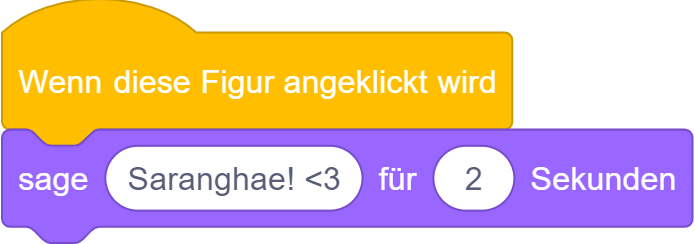
\includegraphics[scale=0.5]{jungkook_script.png}
    \caption[A \scratch{} script controlling the sprite]{\label{fig:script} The program that controls the sprite.}
\end{figure}

\begin{figure}[t]
    \centering
    \subfigure[Sprite in front of a background]{
        \begin{minipage}[t]{0.4\columnwidth}
            \centering
            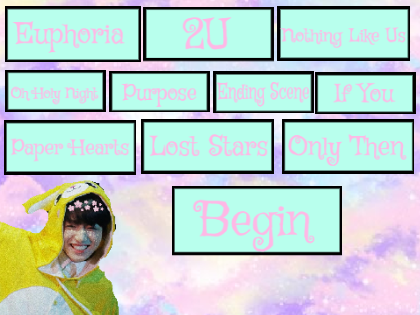
\includegraphics[scale=0.5]{jungkook_stage.png}
        \end{minipage}
    }
    \hfill
    \subfigure[Sprite responding to the clicked event]{
        \begin{minipage}[t]{0.4\columnwidth}
            \centering
            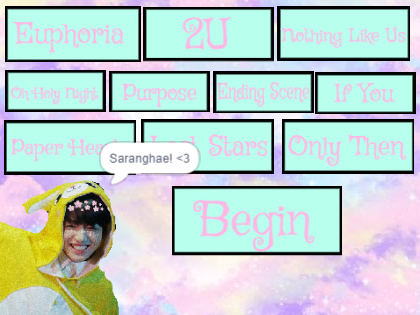
\includegraphics[scale=0.5]{jungkook_stage_action.png}
        \end{minipage}
    }
    \caption[A \scratch{} stage and sprite that respond to events]{\label{fig:sprite}Picture of the sprite on its stage and its reaction after the executed event.}
    \vspace{-1em}
\end{figure}

\subsection{The Static \scratch{} Code Analyser \litterbox{}}\label{subsec:litterbox}
\litterbox{}\footnote{\url{https://gitlab.infosun.fim.uni-passau.de/se2/litterbox}, last accessed August 19, 2020} is a static code analysis tool for detecting bugs in \scratch{} projects where \scratch{} code is saved as a JSON file and downloaded, for example using the \scratch{} REST API\footnote{\url{https://projects.scratch.mit.edu}, last accessed August 20, 2020}. \litterbox{} then creates an abstract syntax tree (AST) for a \scratch{} project. The occurrence of bugs in code is mostly the consequence of recurring bad code writing habits. With the help of \litterbox{} these bug patterns and code smells can be filtered and analysed in order to correct the found bugs and avoid similar mistakes in the future. \litterbox{} is developed at the Chair of Software Engineering II and the Didactics of Informatics of the University of Passau and is the foundation for the analysis of \scratch{} programs with n-gram models in this bachelor's thesis. 


\section{N-gram Language Model}\label{sec:language-models}
Statistical language models, in its essence, are the type of models that assign probabilities to the sequences of words. The \ngram{} is the simplest model that assigns probabilities to sentences and sequences of words. You can think of an N-gram as the sequence of N words, by that notion, a 2-gram (or bigram) is a two-word sequence of words like 'please read', 'read very', or 'very carefully', and a 3-gram (or trigram) is a three-word sequence of words like 'please read very', or 'read very carefully'.

\subsection{Probability Calculation of N-grams}\label{subsec:ngram}
%TODO Explain Markov chain and probability calculation

\subsection{N-gram Model Configuration}\label{subsec:ngram}
There are five key factors that affect the amount of bugs that a language model can find. These are the important \textit{configuration parameters} that need to be set in order to achieve optimal results:  

\begin{definition}[Gram Size]\label{def:gram_size}
    %
    ``The size of an n-gram model. Different gram sizes enable the model to use different internal probabilities to calculate the probabilities of \hyperref[def:token]{token} sequences.''~\cite{bugram}
    %
\end{definition}

\begin{definition}[Sequence Length]\label{def:sequence_length}
    %
    ``The length of token sequences to be considered when building n-gram models and detecting bugs. Different sequence lengths enable the model to capture different program scenarios and further affect the performance of the bug detection.''~\cite{bugram}
    %
\end{definition}

\begin{definition}[Reporting Size]\label{def:reporting_size}
    %
    ``The number of sequences, in the bottom of the ranked list, which will be reported as bugs. An appropriate number may reduce the amount of false positives.''~\cite{bugram}
    %
\end{definition}

\begin{definition}[Minimum Token Occurrence]\label{def:minimum_token_occurrence}
    %
    ``The minimum number of times a token must occur in the code to be included in an n-gram model. An appropriate value helps to filter out \hyperref[def:token]{token} sequences that use unusual/special methods, thus have low probabilities but are not bugs.''~\cite{bugram}
    %
\end{definition}

\begin{definition}[Probability Threshold]\label{def:probability_threshold}
    %
    ``If a \hyperref[def:token]{token} sequence does not reach this probability threshold, it can be considered a bug or unusual occurrence.''
    %
\end{definition}

%TODO Explain n-gram model
